\documentclass[a4paper,oneside,12pt]{report}
\usepackage{fontspec}
\usepackage{setspace}
\usepackage{graphicx}
\usepackage{titling}
\usepackage{geometry}
\usepackage{listings}
\usepackage{xcolor}
\usepackage{float}
\usepackage{hyperref}
\usepackage{indentfirst}
\usepackage{url}
\usepackage{fancyhdr}
\usepackage{tocloft}
\usepackage{bookmark}
\usepackage{booktabs}
\usepackage{caption}

\setmainfont{TeX Gyre Termes}
\onehalfspacing
\geometry{left=3cm, right=2.5cm, top=2cm, bottom=2.5cm}
\sloppy

\definecolor{codegreen}{rgb}{0,0.6,0}
\definecolor{codegray}{rgb}{0.5,0.5,0.5}
\definecolor{codepurple}{rgb}{0.58,0,0.82}
\definecolor{backcolour}{rgb}{0.95,0.95,0.92}
\definecolor{darkblue}{rgb}{0,0,0.6}

\lstdefinestyle{commonstyle}{
    backgroundcolor=\color{backcolour},
    breakatwhitespace=false,
    breaklines=true,
    captionpos=b,
    keepspaces=true,
    numbers=left,
    numbersep=5pt,
    showspaces=false,
    showstringspaces=false,
    showtabs=false,
    tabsize=2,
    frame=single,
    basicstyle=\ttfamily\footnotesize,
    numberstyle=\tiny\color{codegray},
    columns=flexible,
    postbreak=\mbox{\textcolor{red}{$\hookrightarrow$}\space},
    breakindent=0pt,
    breakautoindent=false
}
\lstdefinestyle{bashstyle}{
    style=commonstyle,
    language=bash,
    commentstyle=\color{codegreen},
    keywordstyle=\color{darkblue},
    stringstyle=\color{codepurple}
}
\lstdefinestyle{yamlstyle}{
    style=commonstyle,
    commentstyle=\color{codegreen},
    keywordstyle=\color{darkblue},
    stringstyle=\color{codepurple}
}
\lstdefinestyle{jsstyle}{
    style=commonstyle,
    commentstyle=\color{codegreen},
    keywordstyle=\color{darkblue},
    stringstyle=\color{codepurple}
}
\lstdefinestyle{phpstyle}{
    style=commonstyle,
    commentstyle=\color{codegreen},
    keywordstyle=\color{darkblue},
    stringstyle=\color{codepurple}
}

\newcommand{\customfbox}[1]{%
  \setlength{\fboxsep}{0pt}%
  \setlength{\fboxrule}{0.5pt}%
  \fcolorbox{black}{white}{#1}%
}
\renewcommand{\figurename}{Gambar}
\renewcommand{\thefigure}{\arabic{figure}}
\hypersetup{
    colorlinks=true,
    linkcolor=black,
    filecolor=black,
    urlcolor=black,
    citecolor=black,
    pdftitle={Laporan KEPL Pertemuan 4},
    pdfpagemode=FullScreen,
    breaklinks=true
}
\pagestyle{fancy}
\fancyhf{}
\fancyfoot[C]{\thepage}
\renewcommand{\headrulewidth}{0pt}
\fancypagestyle{plain}{
    \fancyhf{}
    \fancyfoot[C]{\thepage}
    \renewcommand{\headrulewidth}{0pt}
}
\renewcommand{\contentsname}{Daftar Isi}
\renewcommand{\bibname}{Daftar Pustaka}
\renewcommand{\thechapter}{}
\renewcommand{\chaptername}{}
\renewcommand{\thesection}{\arabic{chapter}.\arabic{section}}
\renewcommand{\thesubsection}{\thesection.\arabic{subsection}}
\setcounter{secnumdepth}{3}
\setcounter{tocdepth}{3}
\renewcommand{\cftchapdotsep}{\cftdotsep}
\renewcommand{\cftchapleader}{\cftdotfill{\cftchapdotsep}}
\setlength{\cftchapindent}{0em}
\setlength{\cftsecindent}{2em}
\setlength{\cftsubsecindent}{4em}
\setlength{\cftchapnumwidth}{0em}
\setlength{\cftsecnumwidth}{2.5em}
\setlength{\cftsubsecnumwidth}{3.2em}
\renewcommand{\cftchappresnum}{}
\renewcommand{\cftchapaftersnum}{}
\newcommand{\tocboldsection}[1]{%
  \protect\renewcommand{\protect\cftchapfont}{\protect\bfseries}%
  #1%
  \protect\renewcommand{\protect\cftchapfont}{}%
}

\begin{document}

\newgeometry{left=3cm, right=2.5cm, top=2.5cm, bottom=3cm}
\begin{titlingpage}
\begin{spacing}{1}
\begin{center}
\vspace*{0.2cm}
{\large \textbf{\MakeUppercase{Laporan Praktikum}}} \\[0.4cm]
{\large \textbf{\MakeUppercase{Konstruksi dan Evolusi Perangkat Lunak}}} \\[0.4cm]
{\large \textbf{\MakeUppercase{Pertemuan 4}}} \\[0.4cm]
{\large \textbf{\MakeUppercase{CI/CD untuk Vue.js}}} \\[1.5cm]


\includegraphics[height=7cm]{images/UGM.png} \\[0.7cm]

{\normalsize \textbf{Disusun oleh:}} \\[0.4cm]
\begin{tabular}{@{}l l @{}}
  \textbf{Nama}           & : Hafidz Rizqullah Prasetya \\
  \textbf{NIM}            & : 24/535493/SV/24243 \\
  \textbf{Kelas}          & : PL5A1 \\
  \textbf{Dosen Pengampu} & : Galih Malela Damaraji \\
\end{tabular} \\[1.2cm]

{\normalsize \textbf{PROGRAM STUDI D-IV}} \\[0.2cm]
{\normalsize \textbf{TEKNOLOGI REKAYASA PERANGKAT LUNAK}} \\[0.2cm]
{\normalsize \textbf{DEPARTEMEN TEKNIK ELEKTRO DAN INFORMATIKA}} \\[0.2cm]
{\normalsize \textbf{SEKOLAH VOKASI}} \\[0.2cm]
{\normalsize \textbf{UNIVERSITAS GADJAH MADA}} \\[0.2cm]
{\normalsize \textbf{YOGYAKARTA}} \\[0.2cm]
{\normalsize \textbf{2026}} \\[1.2cm]
\end{center}
\end{spacing}
\end{titlingpage}
\restoregeometry

\thispagestyle{empty}
\clearpage
\stepcounter{page}
\thispagestyle{empty}

\addcontentsline{toc}{chapter}{Daftar Isi}
\tableofcontents
\clearpage

\pagenumbering{arabic}
\setcounter{page}{3}

\chapter[Tujuan Praktikum]{Tujuan Praktikum}
Sesuai arahan pada pertemuan keempat dan deskripsi tugas di Google Classroom \textit{Konstruksi dan Evolusi Perangkat Lunak 2026}, tujuan praktikum ini adalah:
\begin{enumerate}
   \item Mahasiswa mampu menyediakan satu endpoint JSON dari tabel CRUD pada Laravel dan memastikan aplikasi Vue dapat mengaksesnya.
   \item Mahasiswa mampu membuat aplikasi Vue 3 dengan minimal dua halaman ber-router yang mengambil alamat API dari variabel lingkungan.
   \item Mahasiswa mampu menyusun workflow empat job untuk frontend (\texttt{lint}, \texttt{test}, \texttt{build}, \texttt{deploy}) yang dirangkai dengan \texttt{needs:} dan memakai \texttt{npm ci} serta cache \texttt{npm}.
   \item Mahasiswa mampu mengoper hasil build ke job deploy tanpa menjalankan build ulang, dan menampilkan isi direktori \texttt{dist}.
   \item Mahasiswa mampu menulis minimal satu unit test Vitest yang lulus di GitHub Actions tanpa Laravel berjalan.
   \item Mahasiswa mampu membuktikan bahwa Pull Request melewati tahap deploy dan pipeline berhenti ketika satu test sengaja digagalkan.
\end{enumerate}

\clearpage

\chapter{Dasar Teori}

\section{Single Page Application dan Vue 3}
Vue 3 adalah kerangka kerja JavaScript untuk membangun antarmuka yang reaktif \cite{vue-docs}. Pada aplikasi satu halaman, perpindahan antar halaman tidak memuat ulang dokumen, melainkan ditangani oleh \textit{router} di sisi klien. Vue Router memetakan alamat ke komponen sehingga satu berkas HTML dapat melayani beberapa halaman \cite{vue-router}.

\section{Memisahkan Alamat API dari Kode}
Menuliskan alamat API langsung di dalam kode menyulitkan perpindahan antara lingkungan lokal dan produksi. Vite menyediakan variabel lingkungan berawalan \texttt{VITE\_} yang dibaca saat build dan diakses lewat \texttt{import.meta.env} \cite{vite-env}. Dengan pola ini, alamat backend cukup diganti di berkas \texttt{.env} tanpa mengubah kode sumber.

\section{CORS pada API Laravel}
CORS mengatur izin akses lintas domain di peramban \cite{mdn-cors}. Ketika aplikasi Vue dijalankan di \texttt{localhost:5173} dan API berada di \texttt{127.0.0.1:8001}, keduanya dianggap domain berbeda. Laravel mengatur izin itu lewat berkas \texttt{config/cors.php} yang menentukan jalur, metode, dan asal yang diizinkan \cite{laravel-cors}.

\section{Pipeline Frontend Empat Job}
Workflow frontend mengikuti pola yang sama dengan pipeline backend: setiap job berjalan di mesin bersih dan dirangkai memakai \texttt{needs:} \cite{github-actions}. Pemasangan dependensi memakai \texttt{npm ci} agar versi paket persis mengikuti \texttt{package-lock.json}, dan cache \texttt{npm} mempercepat pemasangan pada job berikutnya \cite{github-node}. Hasil \texttt{npm run build} diunggah sebagai artifact, lalu diunduh job deploy. Karena artifact sudah berisi direktori \texttt{dist}, job deploy tidak perlu menjalankan \texttt{npm run build} lagi \cite{github-artifacts}.

\section{Pengujian Unit dengan Vitest}
Vitest menjalankan pengujian unit untuk proyek Vite \cite{vitest-docs}. Karena pengujian dijalankan di lingkungan Node tanpa backend, logika yang diuji harus mandiri dan tidak bergantung pada Laravel. Pada praktikum ini saya memisahkan logika pemformatan dan peringkasan ke berkas \texttt{src/lib/format.js} supaya dapat diuji tanpa menjalankan server.

\clearpage

\chapter[\tocboldsection{Hasil dan Pembahasan}]{Hasil dan Pembahasan}
Pada bab ini saya menjelaskan pekerjaan untuk Tugas 3 sesuai instruksi di Classroom. Saya melanjutkan repository \texttt{evolusi-pl-535493} dengan menambahkan endpoint JSON di sisi Laravel dan aplikasi Vue 3 di folder \texttt{frontend/}.

\section{Alat dan Bahan}
Alat dan bahan yang digunakan:
\begin{itemize}
    \item Laptop dengan OS Linux, akses internet, dan akun GitHub \texttt{hafidzrizqullahprasetya}.
    \item PHP 8.5.10, Composer 2.10.3, Laravel 13, Node.js 26, npm 11, dan Git.
    \item Repository: \texttt{hafidzrizqullahprasetya/evolusi-pl-535493} (publik) dengan aplikasi Laravel dari pertemuan sebelumnya.
    \item Google Classroom: kelas \textit{Konstruksi dan Evolusi Perangkat Lunak 2026} [875340560422], tugas \textit{Pengumpulan Tugas 3} dengan tenggat 28 September 2026.
\end{itemize}

\section{Endpoint JSON di Laravel}
Saya menambahkan tabel \texttt{tugas} beserta model dan pengendali untuk membacanya. Endpoint yang tersedia ada dua: daftar seluruh tugas dan detail satu tugas. Berkas \texttt{routes/api.php} mendaftarkan keduanya, lalu \texttt{bootstrap/app.php} diarahkan agar memuat berkas rute api tersebut.

\begin{lstlisting}[style=phpstyle,caption={Pengendali daftar tugas.}]
class TugasController extends Controller
{
    public function index(): JsonResponse
    {
        return response()->json([
            'data' => Tugas::query()->orderBy('tenggat')->get(),
        ]);
    }
}
\end{lstlisting}

Hasil pemanggilan endpoint lewat \texttt{curl} terlihat pada Gambar \ref{fig:api-json}. Respons berisi empat tugas contoh dengan kolom \texttt{judul}, \texttt{mata\_kuliah}, \texttt{tenggat}, dan \texttt{selesai}.

\begin{figure}[H]
    \centering
    \customfbox{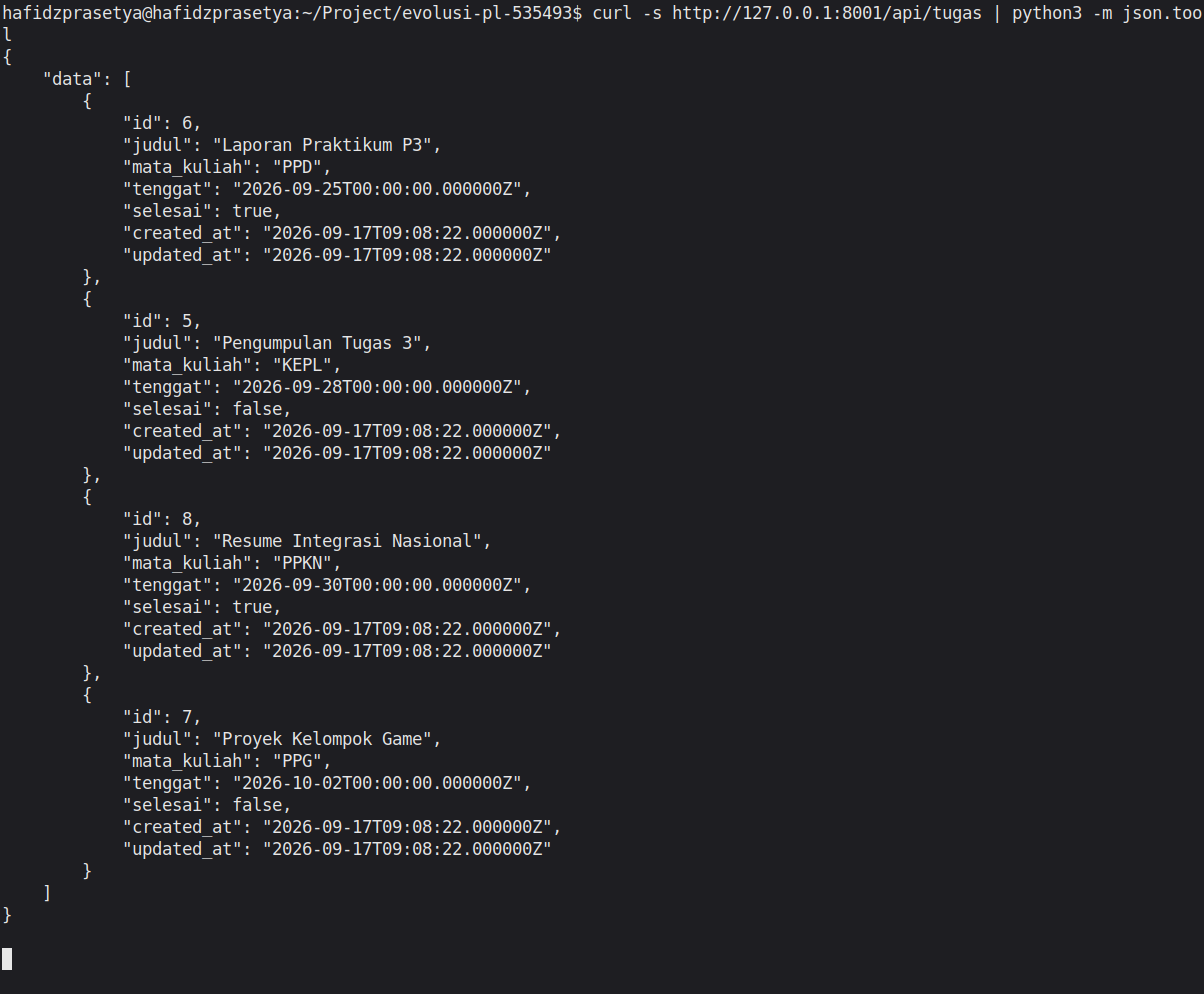
\includegraphics[width=0.95\textwidth]{images/ss-01-api-json.png}}
    \caption{Keluaran \texttt{curl} ke \texttt{/api/tugas} dalam format JSON.}
    \label{fig:api-json}
\end{figure}

\subsection{Mengizinkan Akses dari Vue}
Karena aplikasi Vue berjalan di alamat yang berbeda, saya membuka CORS khusus untuk rute api. Saya menjalankan \texttt{php artisan config:publish cors} untuk menerbitkan berkas konfigurasinya, lalu menyesuaikan jalur, metode, dan asalnya. Pengujian dengan permintaan \textit{preflight} menunjukkan header yang diharapkan:

\begin{lstlisting}[style=bashstyle,caption={Pemeriksaan CORS pada endpoint.}]
curl -s -i http://127.0.0.1:8001/api/tugas | grep -iE 'HTTP/|content-type|access-control'
# HTTP/1.1 200 OK
# Content-Type: application/json
# Access-Control-Allow-Origin: *
\end{lstlisting}

\begin{figure}[H]
    \centering
    \customfbox{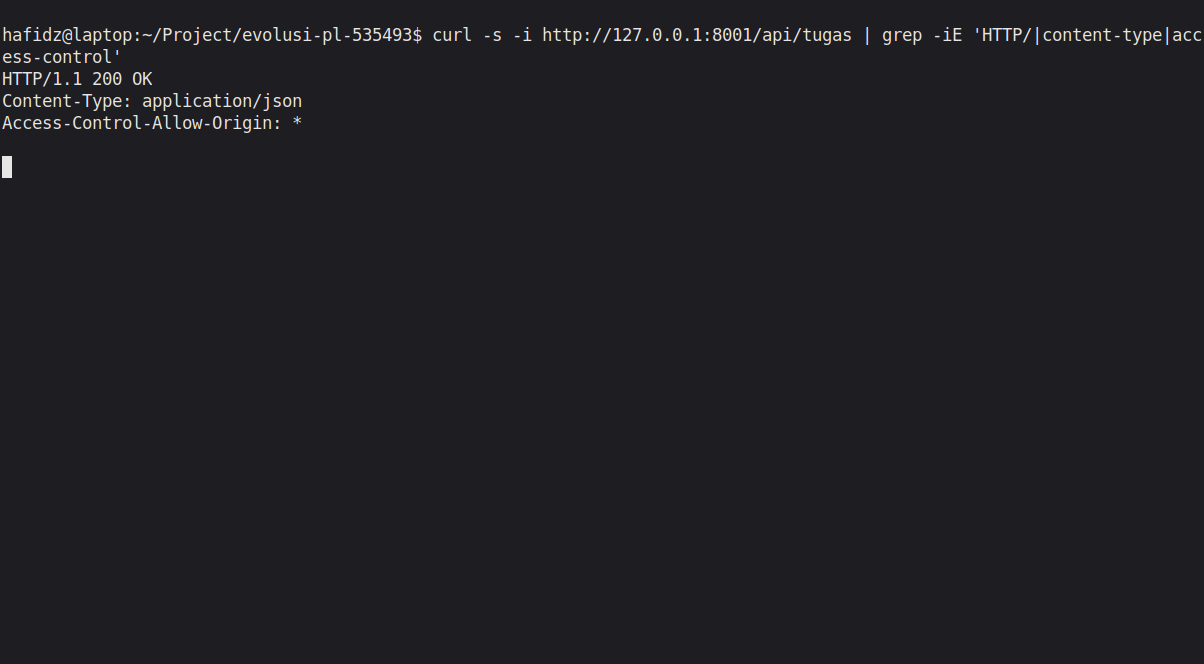
\includegraphics[width=0.95\textwidth]{images/ss-02-api-cors.png}}
    \caption{Respons endpoint yang menyertakan header \texttt{Access-Control-Allow-Origin}.}
    \label{fig:cors}
\end{figure}

\section{Aplikasi Vue 3}
Aplikasi Vue saya letakkan di folder \texttt{frontend/}. Strukturnya memisahkan halaman, router, dan logika yang bisa diuji:

\begin{lstlisting}[style=bashstyle,caption={Struktur folder frontend.}]
frontend/
  index.html
  package.json
  vite.config.js
  eslint.config.js
  src/
    main.js
    App.vue
    router/index.js
    lib/format.js
    lib/api.js
    views/DaftarTugas.vue
    views/Tentang.vue
  tests/format.test.js
\end{lstlisting}

Ada dua halaman ber-router. Halaman \texttt{DaftarTugas.vue} menampilkan data dari Laravel, sedangkan \texttt{Tentang.vue} menjelaskan asal alamat API. Router memetakan keduanya di \texttt{src/router/index.js}:

\begin{lstlisting}[style=jsstyle,caption={Pemetaan rute halaman.}]
const routes = [
  { path: '/', name: 'tugas', component: DaftarTugas },
  { path: '/tentang', name: 'tentang', component: Tentang },
]
\end{lstlisting}

\subsection{Alamat API dari Variabel Lingkungan}
Alamat API tidak ditulis di dalam komponen. Fungsi \texttt{alamatApi} membacanya dari \texttt{import.meta.env.VITE\_API\_URL}, dengan nilai cadangan \texttt{/api} bila variabelnya kosong:

\begin{lstlisting}[style=jsstyle,caption={Pembacaan alamat API dari variabel lingkungan.}]
export function alamatApi(dasar) {
  const nilai = dasar ?? import.meta.env.VITE_API_URL

  if (!nilai) {
    return '/api'
  }

  return nilai.replace(/\/+$/, '')
}
\end{lstlisting}

Nilai variabelnya dicatat pada \texttt{frontend/.env.example} sebagai \texttt{VITE\_API\_URL=http://127.0.0.1:8000/api}, sehingga pengguna lain cukup menyalin berkas itu menjadi \texttt{.env} dan menyesuaikan alamatnya.

\section{Workflow Frontend Empat Job}
Workflow \texttt{.github/workflows/frontend.yml} berisi empat job berurutan: \texttt{lint}, \texttt{test}, \texttt{build}, dan \texttt{deploy}. Job \texttt{lint} dan \texttt{test} memakai \texttt{npm ci} dengan cache \texttt{npm} yang diarahkan ke \texttt{frontend/package-lock.json}. Pemeriksaan gaya kode pada job \texttt{lint} memakai ESLint \cite{eslint-docs}. Job \texttt{build} mengunggah direktori \texttt{frontend/dist} sebagai artifact, dan job \texttt{deploy} mengunduh artifact itu tanpa menjalankan \texttt{npm run build} lagi.

\begin{lstlisting}[style=yamlstyle,caption={Workflow empat job pada \texttt{frontend.yml}.}]
name: Frontend

on:
  push:
    branches: ['**']
    paths: ['frontend/**', '.github/workflows/frontend.yml']
  pull_request:
    paths: ['frontend/**', '.github/workflows/frontend.yml']

jobs:
  lint:
    name: Lint
    runs-on: ubuntu-latest
    steps:
      - name: Ambil kode
        uses: actions/checkout@v4

      - name: Siapkan Node
        uses: actions/setup-node@v4
        with:
          node-version: '22'
          cache: 'npm'
          cache-dependency-path: frontend/package-lock.json

      - name: Pasang dependensi
        working-directory: frontend
        run: npm ci

      - name: Periksa gaya kode
        working-directory: frontend
        run: npm run lint

  test:
    name: Test
    needs: lint
    runs-on: ubuntu-latest
    steps:
      - name: Ambil kode
        uses: actions/checkout@v4

      - name: Siapkan Node
        uses: actions/setup-node@v4
        with:
          node-version: '22'
          cache: 'npm'
          cache-dependency-path: frontend/package-lock.json

      - name: Pasang dependensi
        working-directory: frontend
        run: npm ci

      - name: Jalankan pengujian
        working-directory: frontend
        run: npm test

  build:
    name: Build
    needs: test
    runs-on: ubuntu-latest
    steps:
      - name: Ambil kode
        uses: actions/checkout@v4

      - name: Siapkan Node
        uses: actions/setup-node@v4
        with:
          node-version: '22'
          cache: 'npm'
          cache-dependency-path: frontend/package-lock.json

      - name: Pasang dependensi
        working-directory: frontend
        run: npm ci

      - name: Bangun aplikasi
        working-directory: frontend
        run: npm run build

      - name: Simpan hasil build
        uses: actions/upload-artifact@v4
        with:
          name: dist
          path: frontend/dist
          retention-days: 1

  deploy:
    name: Deploy
    needs: build
    if: github.ref == 'refs/heads/main' && github.event_name == 'push'
    runs-on: ubuntu-latest
    environment: production
    steps:
      - name: Ambil hasil build
        uses: actions/download-artifact@v4
        with:
          name: dist
          path: dist

      - name: Tampilkan isi dist
        run: |
          ls -R dist
          echo "--- isi index.html ---"
          cat dist/index.html
\end{lstlisting}

Pada run terakhir di \texttt{main}, keempat job hijau setelah deploy produksi disetujui:

\begin{lstlisting}[style=bashstyle,caption={Keempat job frontend hijau.}]
gh run view 35203079450 --json jobs --jq '.jobs[] | "\(.name): \(.conclusion)"'
# Lint: success
# Test: success
# Build: success
# Deploy: success
\end{lstlisting}

\begin{figure}[H]
    \centering
    \customfbox{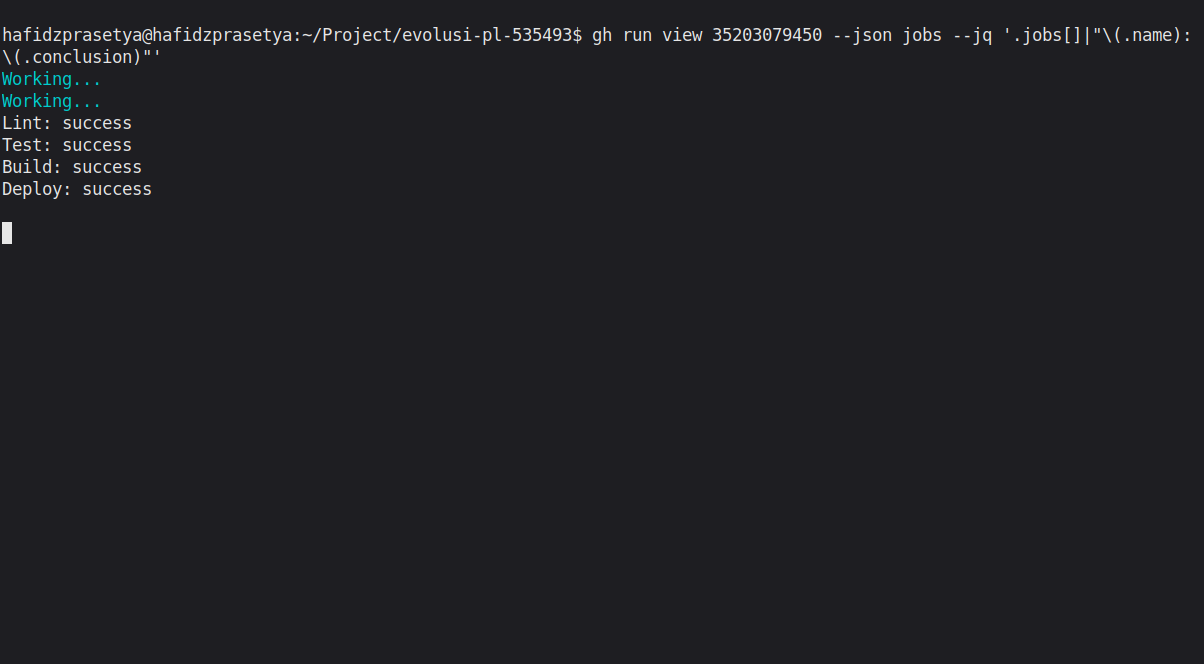
\includegraphics[width=0.95\textwidth]{images/ss-03-frontend-4job.png}}
    \caption{Keempat job workflow frontend hijau pada run di \texttt{main}.}
    \label{fig:frontend-4job}
\end{figure}

\subsection{Deploy Dilewati pada Pull Request}
Sama seperti pipeline backend, job \texttt{deploy} diberi syarat hanya berjalan dari branch \texttt{main} pada kejadian \texttt{push}. Karena itu, ketika pekerjaan berada di branch fitur atau Pull Request, job \texttt{deploy} terlewati sementara lint, test, dan build tetap berjalan:

\begin{lstlisting}[style=bashstyle,caption={Deploy terlewati pada push ke branch fitur.}]
gh run view 35202752695 --json jobs --jq '.jobs[] | "\(.name): \(.conclusion)"'
# Lint: success
# Test: success
# Build: success
# Deploy: skipped
\end{lstlisting}

\begin{figure}[H]
    \centering
    \customfbox{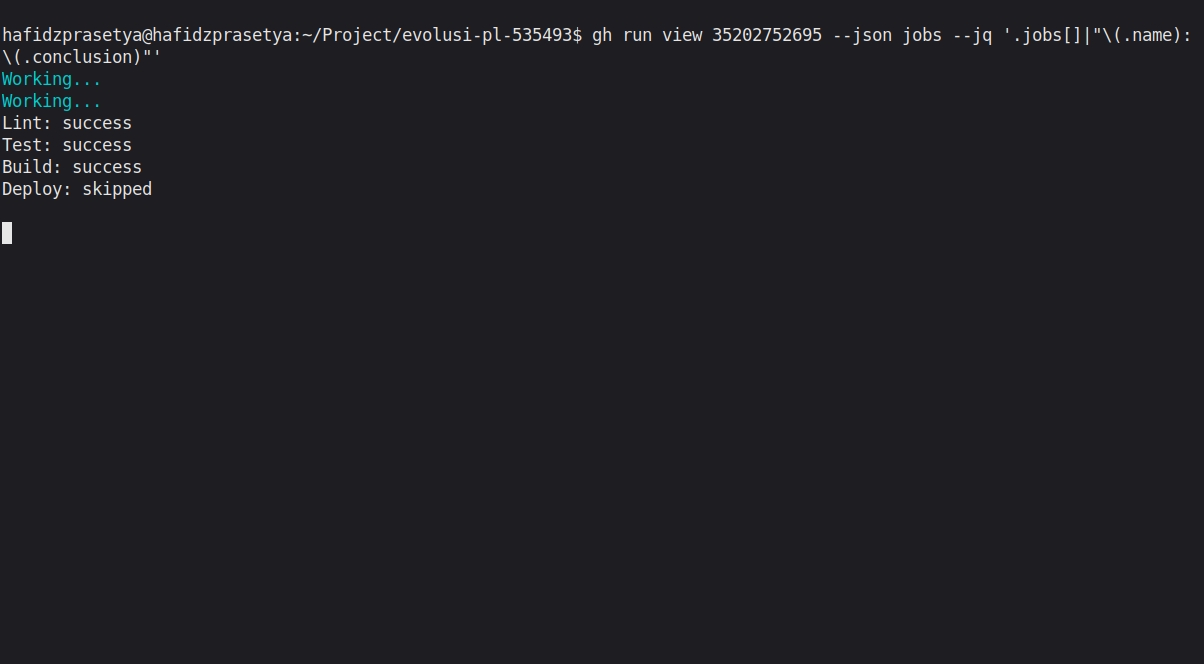
\includegraphics[width=0.95\textwidth]{images/ss-04-deploy-skipped.png}}
    \caption{Push ke branch fitur menjalankan lint, test, dan build, sementara deploy terlewati.}
    \label{fig:deploy-skipped}
\end{figure}

\subsection{Isi Direktori \texttt{dist} di Job Deploy}
Job \texttt{deploy} menampilkan isi direktori \texttt{dist} ke log supaya terlihat bahwa berkas hasil build benar-benar sampai ke job itu. Artifact diunduh lebih dulu, lalu isinya dicetak:

\begin{lstlisting}[style=bashstyle,caption={Langkah job deploy.}]
- name: Ambil hasil build
  uses: actions/download-artifact@v4
  with:
    name: dist
    path: dist
- name: Tampilkan isi dist
  run: |
    ls -R dist
    echo "--- isi index.html ---"
    cat dist/index.html
\end{lstlisting}

\begin{figure}[H]
    \centering
    \customfbox{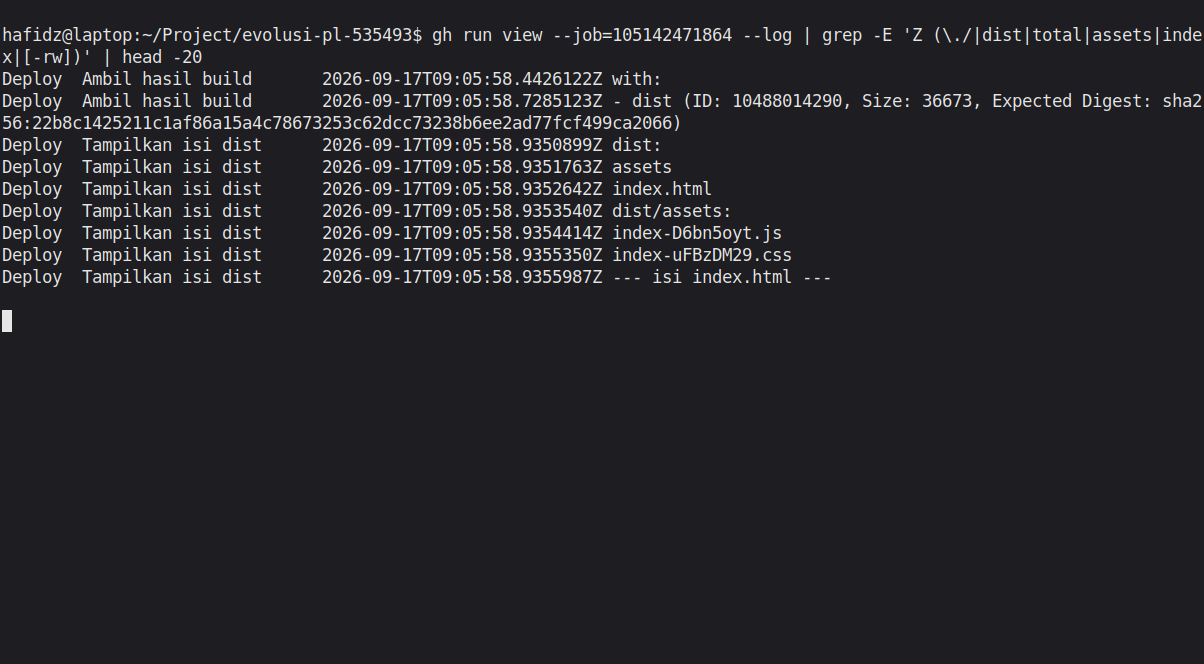
\includegraphics[width=0.95\textwidth]{images/ss-06-log-deploy.png}}
    \caption{Log job \texttt{Deploy} yang menampilkan isi direktori \texttt{dist} hasil build.}
    \label{fig:log-deploy}
\end{figure}

\section{Unit Test Vitest}
Logika pemformatan tanggal dan peringkasan tugas saya taruh di \texttt{src/lib/format.js} agar bisa diuji tanpa backend. Berkas \texttt{tests/format.test.js} menguji fungsi tersebut dengan tujuh kasus, termasuk tanggal kosong, tanggal tidak valid, dan daftar tugas kosong. Pengujian dijalankan dengan \texttt{npm test}:

\begin{lstlisting}[style=bashstyle,caption={Hasil pengujian Vitest di laptop.}]
npm test
# Test Files  1 passed (1)
#      Tests  7 passed (7)
\end{lstlisting}

\begin{figure}[H]
    \centering
    \customfbox{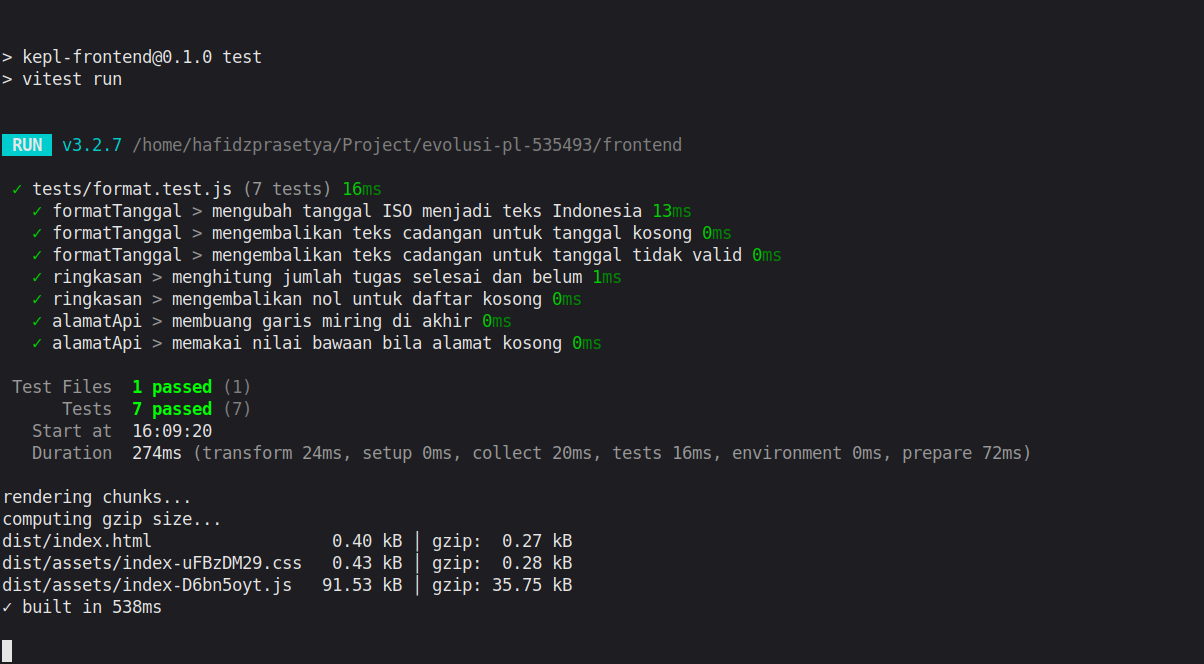
\includegraphics[width=0.95\textwidth]{images/ss-07-lint-test-build.png}}
    \caption{Pemeriksaan gaya kode, pengujian Vitest, dan build yang dijalankan di laptop.}
    \label{fig:lint-test-build}
\end{figure}

\section{Bukti Pipeline Berhenti Saat Test Gagal}
Sesuai instruksi tugas, saya sengaja menggagalkan satu test untuk membuktikan pipeline berhenti. Nilai harapan pada kasus uji peringkasan saya ubah dari 2 menjadi 9, lalu push. Job \texttt{test} gagal, dan job \texttt{build} serta \texttt{deploy} otomatis terlewati karena \texttt{needs:} tidak terpenuhi.

\begin{lstlisting}[style=bashstyle,caption={Pipeline frontend merah pada test yang sengaja digagalkan.}]
gh run view 35202565338 --json jobs --jq '.jobs[] | "\(.name): \(.conclusion)"'
# Lint: success
# Test: failure
# Build: skipped
# Deploy: skipped

# expected { total: 3, selesai: 2, belum: 1 } to deeply equal
#   { total: 3, selesai: 9, belum: 1 }
# Tests  1 failed | 6 passed (7)
\end{lstlisting}

\begin{figure}[H]
    \centering
    \customfbox{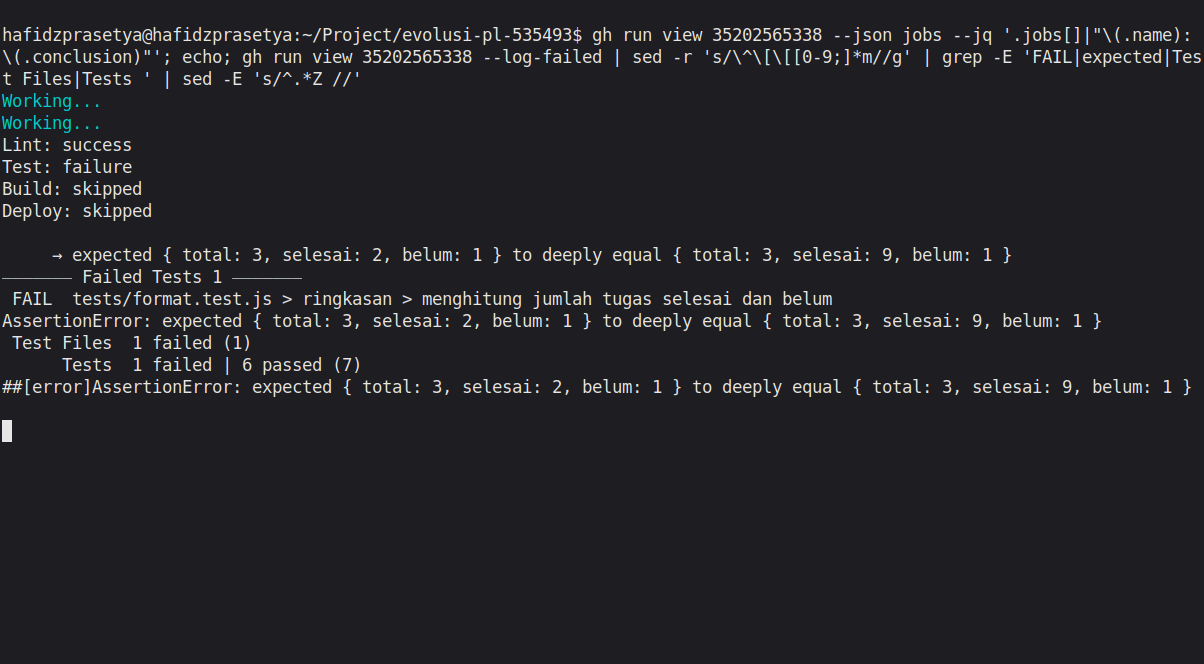
\includegraphics[width=0.95\textwidth]{images/ss-05-vitest-merah.png}}
    \caption{Satu test Vitest yang digagalkan menghentikan pipeline: build dan deploy terlewati.}
    \label{fig:vitest-merah}
\end{figure}

Setelah bukti itu tersimpan, saya mengembalikan nilai harapan ke 2 dan push lagi. Pipeline kembali hijau pada commit berikutnya.

\clearpage

\chapter{Kesimpulan}
Berdasarkan praktikum pada Pertemuan 4, dapat disimpulkan beberapa hal:

\begin{enumerate}
    \item Endpoint JSON \texttt{/api/tugas} berhasil disediakan dan dapat diakses aplikasi Vue setelah CORS dibuka untuk rute api.
    \item Aplikasi Vue 3 di folder \texttt{frontend/} memiliki dua halaman ber-router, dan alamat API diambil dari \texttt{VITE\_API\_URL} alih-alih ditulis di dalam kode.
    \item Workflow frontend berisi empat job (\texttt{lint}, \texttt{test}, \texttt{build}, \texttt{deploy}) yang dirangkai dengan \texttt{needs:} dan memakai \texttt{npm ci} beserta cache \texttt{npm}.
    \item Hasil build dioper ke job deploy lewat artifact, dan job deploy tidak menjalankan build ulang serta menampilkan isi direktori \texttt{dist} ke log.
    \item Deploy terbukti hanya berjalan dari \texttt{main}; pada Pull Request dan branch fitur, job itu terlewati.
    \item Pipeline terbukti berhenti ketika satu test Vitest sengaja digagalkan, lalu kembali hijau setelah kesalahan diperbaiki.
\end{enumerate}

Dengan ini alur CI/CD repository \texttt{evolusi-pl-535493} sudah mencakup sisi backend dan frontend, dengan deploy yang terjaga pada branch \texttt{main}.

\clearpage
\addcontentsline{toc}{chapter}{Daftar Pustaka}
\renewcommand{\bibname}{Daftar Pustaka}
\begin{thebibliography}{99}
    \bibitem{vue-docs} Vue.js, ``Vue.js Documentation.'' [Online]. Tersedia: \url{https://vuejs.org/guide/introduction.html}.

    \bibitem{vue-router} Vue.js, ``Vue Router.'' [Online]. Tersedia: \url{https://router.vuejs.org/}.

    \bibitem{vite-env} Vite, ``Env Variables and Modes.'' [Online]. Tersedia: \url{https://vite.dev/guide/env-and-mode}.

    \bibitem{mdn-cors} MDN Web Docs, ``Cross-Origin Resource Sharing (CORS).'' [Online]. Tersedia: \url{https://developer.mozilla.org/en-US/docs/Web/HTTP/CORS}.

    \bibitem{laravel-cors} Laravel, ``Laravel Documentation.'' [Online]. Tersedia: \url{https://laravel.com/docs}.

    \bibitem{github-actions} GitHub Docs, ``Understanding GitHub Actions.'' [Online]. Tersedia: \url{https://docs.github.com/en/actions/learn-github-actions/understanding-github-actions}.

    \bibitem{github-node} GitHub Docs, ``Building and testing Node.js.'' [Online]. Tersedia: \url{https://docs.github.com/en/actions/automating-builds-and-tests/building-and-testing-nodejs}.

    \bibitem{github-artifacts} GitHub Docs, ``Storing and sharing data from a workflow.'' [Online]. Tersedia: \url{https://docs.github.com/en/actions/using-workflows/storing-workflow-data-as-artifacts}.

    \bibitem{vitest-docs} Vitest, ``Vitest Documentation.'' [Online]. Tersedia: \url{https://vitest.dev/guide/}.

    \bibitem{eslint-docs} ESLint, ``ESLint Documentation.'' [Online]. Tersedia: \url{https://eslint.org/docs/latest/}.

\end{thebibliography}

\end{document}
